% arara: pdflatex
% arara: biber
% arara: pdflatex
% arara: pdflatex 
% Chandra Images by Category: Supernovas & Supernova Remnants
% https://chandra.harvard.edu/photo/category/snr.html

\documentclass[a4paper,12pt]{extarticle}
%\documentclass{article}
\usepackage{graphicx}
\RequirePackage[l2tabu,orthodox]{nag} % Раскомментировав, можно в логе получать рекомендации относительно правильного использования пакетов и предупреждения об устаревших и нерекомендуемых пакетах
% \documentclass[a4paper,14pt]{extarticle}
\usepackage[left=1.5 cm,right=1.6cm,top=1.5cm,bottom=2.5cm]{geometry}

%%% Mathematical packages %%%
\usepackage{amsthm,amsmath,amscd} % Математические дополнения от AMS
\usepackage{amsfonts,amssymb}     % Математические дополнения от AMS
\usepackage{mathtools}            % Добавляет окружение multlined
\usepackage{mathtext}
\usepackage{cancel}

\usepackage{textcomp}

\RequirePackage{ifxetex, ifluatex}
\ifxetex
  % https://tex.stackexchange.com/a/38631
  \renewcommand{\mathbf}{\ensuremath{\symbf}}
  \usepackage{unicode-math}
  \usepackage{polyglossia}                        % Поддержка многоязычности (fontspec подгружается автоматически)
 % \setmainlanguage[babelshorthands=true]{russian} % Язык по-умолчанию русский с поддержкой приятных команд пакета babel
  \setotherlanguage{english}                      % Дополнительный язык = английский (в американской вариации по-умолчанию)
  % Семейство шрифтов Liberation (https://pagure.io/liberation-fonts)
  \setmonofont{LiberationMono}[Scale=0.87]        % моноширинный шрифт
  \newfontfamily\cyrillicfonttt{LiberationMono}[  % моноширинный шрифт для кириллицы
    Scale=0.87]
  \defaultfontfeatures{Ligatures=TeX}             % стандартные лигатуры TeX, замены нескольких дефисов на тире и т. п. Настройки моноширинного шрифта должны идти до этой строки, чтобы при врезках кода программ в коде не применялись лигатуры и замены дефисов
  \setmainfont{LiberationSerif}                   % Шрифт с засечками
  \newfontfamily\cyrillicfont{LiberationSerif}    % Шрифт с засечками для кириллицы
  \setsansfont{LiberationSans}                    % Шрифт без засечек
  \newfontfamily\cyrillicfontsf{LiberationSans}   % Шрифт без засечек для кириллицы

  % fake small capitals
  % https://tex.stackexchange.com/questions/55664/fake-small-caps-with-xetex-fontspec
  \makeatletter
  \newlength\fake@f
  \newlength\fake@c
  \def\textsc#1{%
    \begingroup%
    \xdef\fake@name{\csname\curr@fontshape/\f@size\endcsname}%
    \fontsize{\fontdimen8\fake@name}{\baselineskip}\selectfont%
    \MakeUppercase{#1}%
    \endgroup%
    }
  \makeatother
  % \renewcommand{\textsc}[1]{\fauxschelper#1 \relax\relax}
  % \def\fauxschelper#1 #2\relax{%
  %   \fauxschelphelp#1\relax\relax%
  %   \if\relax#2\relax\else\ \fauxschelper#2\relax\fi%
  %   }
  % \def\Hscale{.83}\def\Vscale{.72}\def\Cscale{1.00}
  % \def\fauxschelphelp#1#2\relax{%
  %   \ifnum`#1>``\ifnum`#1<`\{\scalebox{\Hscale}[\Vscale]{\uppercase{#1}}\else%
  %   \scalebox{\Cscale}[1]{#1}\fi\else\scalebox{\Cscale}[1]{#1}\fi%
  %   \ifx\relax#2\relax\else\fauxschelphelp#2\relax\fi}

\else
  \usepackage[T2A]{fontenc}           % кодировка
  \usepackage[utf8]{inputenc}         % Кодировка utf8
  \usepackage[english,russian]{babel} % Языки: русский, английский
\fi

\usepackage[colorlinks=true,unicode=true]{hyperref}

%%% Other packages %%%
\usepackage{xspace} % пробелы после предопределённых команд
\usepackage{color}
\usepackage{enumitem}
\usepackage{cmap}
\usepackage{array}
\usepackage{braket}
\usepackage{epsfig}
\usepackage{epstopdf}
\usepackage{graphicx}
\usepackage{float}
\usepackage{caption}
\captionsetup{compatibility=false}
\usepackage{subcaption}
\usepackage{indentfirst}
\usepackage{hyphenat}
\usepackage[normalem]{ulem}
\usepackage{wrapfig}
\usepackage{pdfpages}

\graphicspath{{img/}} % Пути к изображениям

%%% Toc %%%
% \setcounter{tocdepth}{4}
% \setcounter{secnumdepth}{4}

%%% Title %%%
% \usepackage{titlesec}
% \titleformat{\section}
% {\normalfont\large\bfseries}{\thesection}{1em}{}

%%% Setup bibliography %%%

\usepackage{csquotes} % biblatex рекомендует его подключать. Пакет для оформления сложных блоков цитирования.
%%% Загрузка пакета с основными настройками %%%
\makeatletter
\usepackage[%
backend=biber,% движок
bibencoding=utf8,% кодировка bib файла
sorting=none,% настройка сортировки списка литературы
style=gost-numeric,% стиль цитирования и библиографии (по ГОСТ)
language=autobib,% получение языка из babel/polyglossia, default: autobib % если ставить autocite или auto, то цитаты в тексте с указанием страницы, получат указание страницы на языке оригинала
autolang=other,% многоязычная библиография
clearlang=true,% внутренний сброс поля language, если он совпадает с языком из babel/polyglossia
defernumbers=true,% нумерация проставляется после двух компиляций, зато позволяет выцеплять библиографию по ключевым словам и нумеровать не из большего списка
sortcites=true,% сортировать номера затекстовых ссылок при цитировании (если в квадратных скобках несколько ссылок, то отображаться будут отсортированно, а не абы как)
movenames=false, % опция разрешает или запрещает перемещение имён в область сведений об ответственности, если количество имён больше трёх.
% не менять местами заголовок и список авторов, если авторов больше четырех
minnames=3, % сокращение списка имён
maxnames=4, % сокращение списка имён
doi=true,% Показывать или нет ссылки на DOI
isbn=false,% Показывать или нет ISBN, ISSN, ISRN
url=false,
eprint=true,
backref=true
]{biblatex}[2016/09/17]
%]{biblatex}
%\ltx@iffilelater{biblatex-gost.def}{2017/05/03}%
{\toggletrue{bbx:gostbibliography}%
\renewcommand*{\revsdnamepunct}{\addcomma}}{}
\makeatother

\DefineBibliographyStrings{english}{docthesis = {dissertation}}
\DefineBibliographyStrings{russian}{docthesis = {диссертация}}

% Custom backref Text
%https://tex.stackexchange.com/questions/196015/custom-backref-text
\DefineBibliographyStrings{english}{
  backrefpage  = {Цит. на с.\adddot},
  backrefpages = {Цит. на с.\adddot},
}
\DefineBibliographyStrings{russian}{
  backrefpage  = {Цит. на с.\adddot},
  backrefpages = {Цит. на с.\adddot},
}
\ifxetex
\else
% Исправление случая неподдержки знака номера в pdflatex
    \DefineBibliographyStrings{russian}{number={\textnumero}}
\fi

% разделитель ; для ссылок
\DeclareMultiCiteCommand{\multicites}[\mkbibbrackets]{\cite}{\addsemicolon\space}

%%% Colors %%%
\usepackage[dvipsnames]{xcolor}

\definecolor{linkcolor}{rgb}{0.08, 0.38, 0.74}
\definecolor{citecolor}{rgb}{0.18, 0.55, 0.34}
\definecolor{urlcolor}{rgb}{0.03, 0.57, 0.82}

\hypersetup{
    linktocpage=true,           % ссылки с номера страницы в оглавлении, списке таблиц и списке рисунков
    colorlinks,                 % ссылки отображаются раскрашенным текстом, а не раскрашенным прямоугольником, вокруг текста
    linkcolor={linkcolor},      % цвет ссылок типа ref, eqref и подобных
    citecolor={citecolor},      % цвет ссылок-цитат
    urlcolor={urlcolor},        % цвет гиперссылок
}

%%% Users commands %%%

\def\stella{\code{STEL\-LA}\xspace}
\def\millimetron{\code{Миллиметрон}\xspace}
\def\mesa{\code{ME\-SA}\xspace}
\def\supremna{\code{SUP\-REM\-NA}\xspace}

\def\araa{Annual Review of Astronomy and Astrophysics}
\def\apj{The Astrophysical Journal}
\def\apjl{The Astrophysical Journal Letters}
\def\apjs{The Astrophysical Journal Supplement}
\def\apss{Astrophysics and Space Science}
\def\azh{Астрон. Журнал}
\def\pazh{Письма в Астрон. Журнал}
\def\pasp{Pub. Astron. Soc. Pacific}
\def\pasa{Pub. Astron. Soc. Australia}
\def\prl{Phys. Rev. Lett}
\def\pre{Phys. Rev. E}
\def\sovast{Soviet Astronomy}
\def\aa{Astronomy and Astrophysics}
\def\aapr{Astronomy and Astrophysics Reviews}
\def\aj{Astronomical Journal}
\def\mnras{MNRAS}
\def\nat{Nature}
\def\ssr{Space Science Reviews}
\def\prd{Phys. Rev. D}
\def\jqsrt{Journal of Quantitative Spectroscopy and Radiative Transfer}

\DeclareRobustCommand{\todo}{\textcolor{red}}

\newcommand{\code}[1]{\texttt{#1}}
% \newcommand{\code}[1]{\textsc{#1}}
\newcommand\vecx[1]{\ifstrequal{#1}{0}{\ensuremath{\mathbf{0}}}{\ensuremath{\boldsymbol{#1}}}}

\newcommand\vecxu{\vecx{u}}



\newcommand{\pb}[1]{\textbf{\color{magenta}PB: #1}}
\newcommand{\iz}[1]{\textbf{\color{orange}IZ: #1}}

\newcommand\nifsx{$^{56}$Ni\xspace}
\newcommand\cofsx{$^{56}$Co\xspace}
\newcommand\fefsx{$^{56}$Fe\xspace}
\newcommand{\rsun}{\ensuremath{R_\odot}\xspace}
\newcommand{\msun}{\ensuremath{M_\odot}}

% 
\def\rej{\ensuremath{R_{\rm ej}}}
\def\mej{\ensuremath{M_{\rm ej}}}
\def\renv{\ensuremath{R_{\rm env}}}
\def\menv{\ensuremath{M_{\rm env}}}

\newcommand\snia{SN\,Ia\xspace}
\newcommand\snib{SN\,Ib\xspace}
\newcommand\snic{SN\,Ic\xspace}
\newcommand\sniib{SN\,IIb\xspace}
\newcommand\sniip{SN\,IIP\xspace}



%%% Add bibliography
\addbibresource{refs_hd.bib}

\begin{document}
\begin{titlepage} 
    \begin{figure}[!htb]
	\centering
	
\includegraphics[width=0.9\textwidth]{Sketch_MSU.png}
	\label{fig:Sketch_MSU}
    \end{figure}
    \begin{center}
    \textbf{\Large  МОСКОВСКИЙ ГОСУДАРСТВЕННЫЙ УНИВЕРСИТЕТ \\
ИМЕНИ М. В. ЛОМОНОСОВА} 
    \end{center}
    \begin{center}
    \end{center}
    \begin{center}
     \text{\Large Факультет космических исследований}
    \end{center}
    \begin{center}
    \end{center}
    \begin{center}
    \end{center}
    \begin{center}
    \text{\Large Курсовая работа\newline}
    
    \text{\Large 
    Моделирование радиоизлучения от сверхновых и их остатков}
    \end{center}
    \vspace{6cm}
    \begin{flushright}
    Выполнил студент 3 курса специалитета Заворохин Илья Владимирович\\
    Научный руководитель: к. ф-м. н. Бакланов Петр Валерьевич
    \end{flushright}
    \vspace{3cm}
    \begin{center}
        Москва, 2024
    \end{center}
\end{titlepage} 


\date{\today}
\tableofcontents
\newpage

\section{Введение}
Исследование сверхновых оказывает огромное влияние на развитие представлений учёных о фундаментальных явлениях происходящих в звёздах, о происхождении тяжёлых элементов, а также для исследования динамики эволюции всей Вселенной. 
Наблюдения вспышек звезд с Земли начались ещё за несколько тысячелетий до нашей эры.
В отличие от вспышек обыкновенных новых звезд вспышки сверхновых в современном состоянии нашей Галактики — явление крайне редкое, происходящее не чаще чем раз в 100 лет. Наиболее яркими были вспышки в 1006 и 1054 годах, сведения о них содержатся в китайских и японских трактатах. В 1572 году вспышку такой звезды в созвездии Кассиопеи наблюдал выдающийся астроном Тихо Браге, последним же, кто следил за явлением сверхновой в созвездии Змееносца в 1604 году, был Иоганн Кеплер. За четыре столетия «телескопической» эры в астрономии подобных вспышек в нашей Галактике не наблюдалось.

Cущественные продвижения в изучении сверхновых начались в середине 20 века, с развитием радиоастрономических наблюдений \cite{Kaplan1966}.  
Впервые космическое радиоизлучение было открыто Карлом Янским в 1931-32 гг. Затем в 1937 году Гроут Ребер, вдохновившись исследованиями Янского, построил параболический радиотелескоп диаметром 9.5 метров. В 1944 году он опубликовал в своей работе первые радиокарты небосвода, где отчетливо были видры центральные области Млечного Пути и яркие радиоисточниики в созвездии Стрельца, Лебедя А, Кассиопеи А, Большого Пса и Корма. 

Основными целями данной работы являются: изучение процессов происходящих во время разлета остатков сверхновых, взаимодействие остатков с межзвездным веществом, а также наблюдение этих процессов в радиодиапазоне. В разделе \ref{sec: Supernovae} описана классификация сверхновых звезд, а также приведено описание радионаблюдений сверхновых. В разделе \ref{sec: Supernova remnants} дано подробное описание каждой стадии разлета, приведены характерные времена каждой стадии, а также приводятся основные соотношения для характеристик остатка. Возможные механизмы возникновения радиоизлучения в космосе описаны в разделе \ref{sec: Radio emission}. Синхротронный механизм, имеющий непосредственное отношение к остаткам сверхновых описан в разделе \ref{sec: Synchrotron}.
Особое значение при рассмотрении взамодействия остатка с межзвездным веществом имеют возникающие в ходе этого ударные волны, идущие как внутрь остатка, так и по внешнему веществу. 
Для знакомства с явлениями ударных волн в газе, были поставлени цели: разобраться с аналитическим рещением классической задачи Римана о распаде произвольного разрыва, а также создать его программную реализацию. На основе написанной программы в дальнешей работе будет возможно осуществление проверки численных решений этой задачи, а также модифицирование условий задачи в сторону более приближенных к реальным физическим явлениям происходящих в астрофизических условиях.Подробное рассмотрение этой части работы дано в приложении \ref{sec: Shockwave}. 

\newpage
%---------------------------------------------------

\section{Сверхновые} \label{sec: Supernovae}
Сверхновая является заключительной стадией жизни некоторых звёзд.{\cite{Shklov1984}} В зависимости от внутреннего состава звезды вспышка может осуществляться разными механизмами и давать при этом разную картину на получаемых данных (кривых блеска). Выделяют 2 основных типа сверхновых: I и II. К I типу относят сверхновые, спектры которых не содержат линий водорода, ко II типу, наоборот, содержащие такие линии. Сверхновые I типа делят на 3 подтипа: Ia (есть кремний), Ib(есть гелий), Ic(нет гелия). Сверхновые II типа по их спектру делят на два подтипа IIb и IIn; по кривой блеска (наличие плато) - IIP и IIL. На рис \ref{fig:light_curves} представлены несколько примеров кривых блеска сверхновых разных типов. 

\begin{figure}[!htb] 
	\centering
	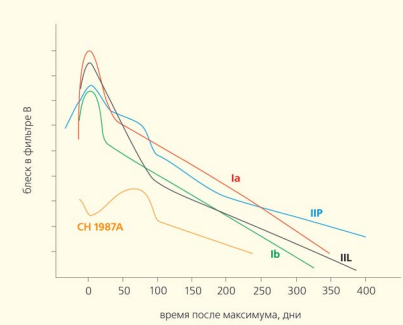
\includegraphics[width=0.7\textwidth]{Характерные кривые блеска.png}
	\caption{
		Примеры характерных кривых блеска для разных типов сверхновых. График из статьи М.В.Пружинской и С.М.Лисакова в журанале Природа №12, 2015 г.
	}
	\label{fig:light_curves}
\end{figure}

В таблице \ref{table: parameters supernova} представлено сравнение параметров сверхновых I и II типов.  Остутствие водорода в звезде перед взрывом сверхновой типа Ia приводит к тому, что сам взрыв существенно отличается от взрывов остальных типов. Причиной возникновения сверхновой типа Ia является термоядерный взрыв, а у всех остальных - гравитационный коллапс. 

\captionof{table}{Средние параметры Сверхновых}
\hskip+1.6cm
\begin{tabular}{|m{6cm}|m{4cm}|m{4cm}|}
    \hline
    Параметр & I тип & II тип \\
    \hline
     Абсолютная величина в максимуме блеска М$_{max}$ & $-19^m$ & $-17..-18^m$ \\
    \hline
     Энергия вспышки & $10^{50}$ эрг & $10^{50}-10^{51}$ эрг \\
    \hline
     Масса звезды предшественника & $\approx 1.5M_\odot$ & $\approx 10M_\odot$ \\
     \hline
     Скорость выброса & $15000-20000$ км/с & $\approx 6000$ км/с \\
     \hline
     Примеры остатков & Тихо (1572), Кеплер (1604), Краб (1006) & Кассиопея А (1947), SN 1993J \\
     \hline
\end{tabular}\label{table: parameters supernova}
\\ \\ \\ \\
Наблюдения остатков сверхновых в разных диапаонах электромагнитных волн (рис. \ref{fig:Crab rafio infra visible} и \ref{fig:Tycho Infra Optic XRay}) позволяет лучше понять как причины их образования, так и все происходящие внутри них процессы.  
\begin{figure}[!htb] 
	\centering
	\includegraphics[width=0.9\textwidth]{Сrab_Radio_Infra_Visible.png}
	\caption{
		Изображения Крабовидной туманности в радио-, инфракрасном и видимом диапазоне
	}
	\label{fig:Crab rafio infra visible}
\end{figure}

\begin{figure}[!htb] 
	\centering
	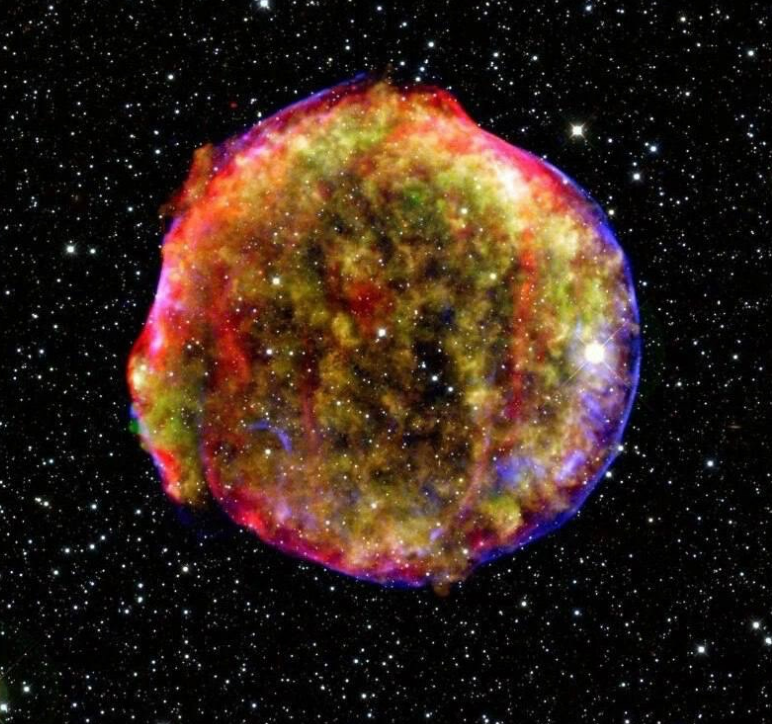
\includegraphics[width=0.5\textwidth]{Tycho_Optic_Infra_XRay.png}
	\caption{
		Комбинированное изображение остатка Тихо в трех диапазонах: инфракрасном, видимом и рентгеновском
	}
	\label{fig:Tycho Infra Optic XRay}
\end{figure}


\section{Радиоизлучениe от cверхновых} \label{sec: Radio emission}
\hspace{1cm} В данной работе основным рассматриваемым диапазоном электромагнитных волн является радиодиапазон.
К нему относятся ЭМ волны с длиной волны ($\lambda$) более 1мм (или частотами до 220 ГГц).




\subsection{Радионаблюдения сверхновых}
Обнаружение радиоизлучения от остатков вспышек сверхновых является важнейшим этапом в истории изучения этих объектов. Исследование радиоизлучения является эффектинвым методом анализа физических условий в расширяющихся оболочках. Далее идет описание основных результатов наблюдения радиоизлучения остатков вспышек сверхновых (\cite{Shklov1984}).\\
\indent В 1948 г. английские радиоастрономы Райл и Смит обнаружили на северном небе в созвездии Кассиопеи необыкновенно яркий источник радиоизлучения, названный ими «Кассиопея А». 
Радиоспектр Кассиопеи А весьма характерен, он хорошо представляется степенным законом:
$$ F_\nu \propto \nu^{-\alpha},$$
где $\nu$ - частота, а $\alpha \approx 0.8$ во всём диапазоне частот от метровых до сантиметровых волн. Велична $\alpha $ называется спектральным индексом, а $F_\nu$ - спектральная плотность потока. Степенной характер является типичным для большинства источников космического радиоизлучения. Такой характер спектра связан с механизмом радиоизлучения (подробнее в разделе \ref{sec: Radio emission}). 
Кассиопея А является прототипом класса остатков, получившего название "богатые кислородом" остатки. 

\begin{figure}[!htb] 
	\centering
	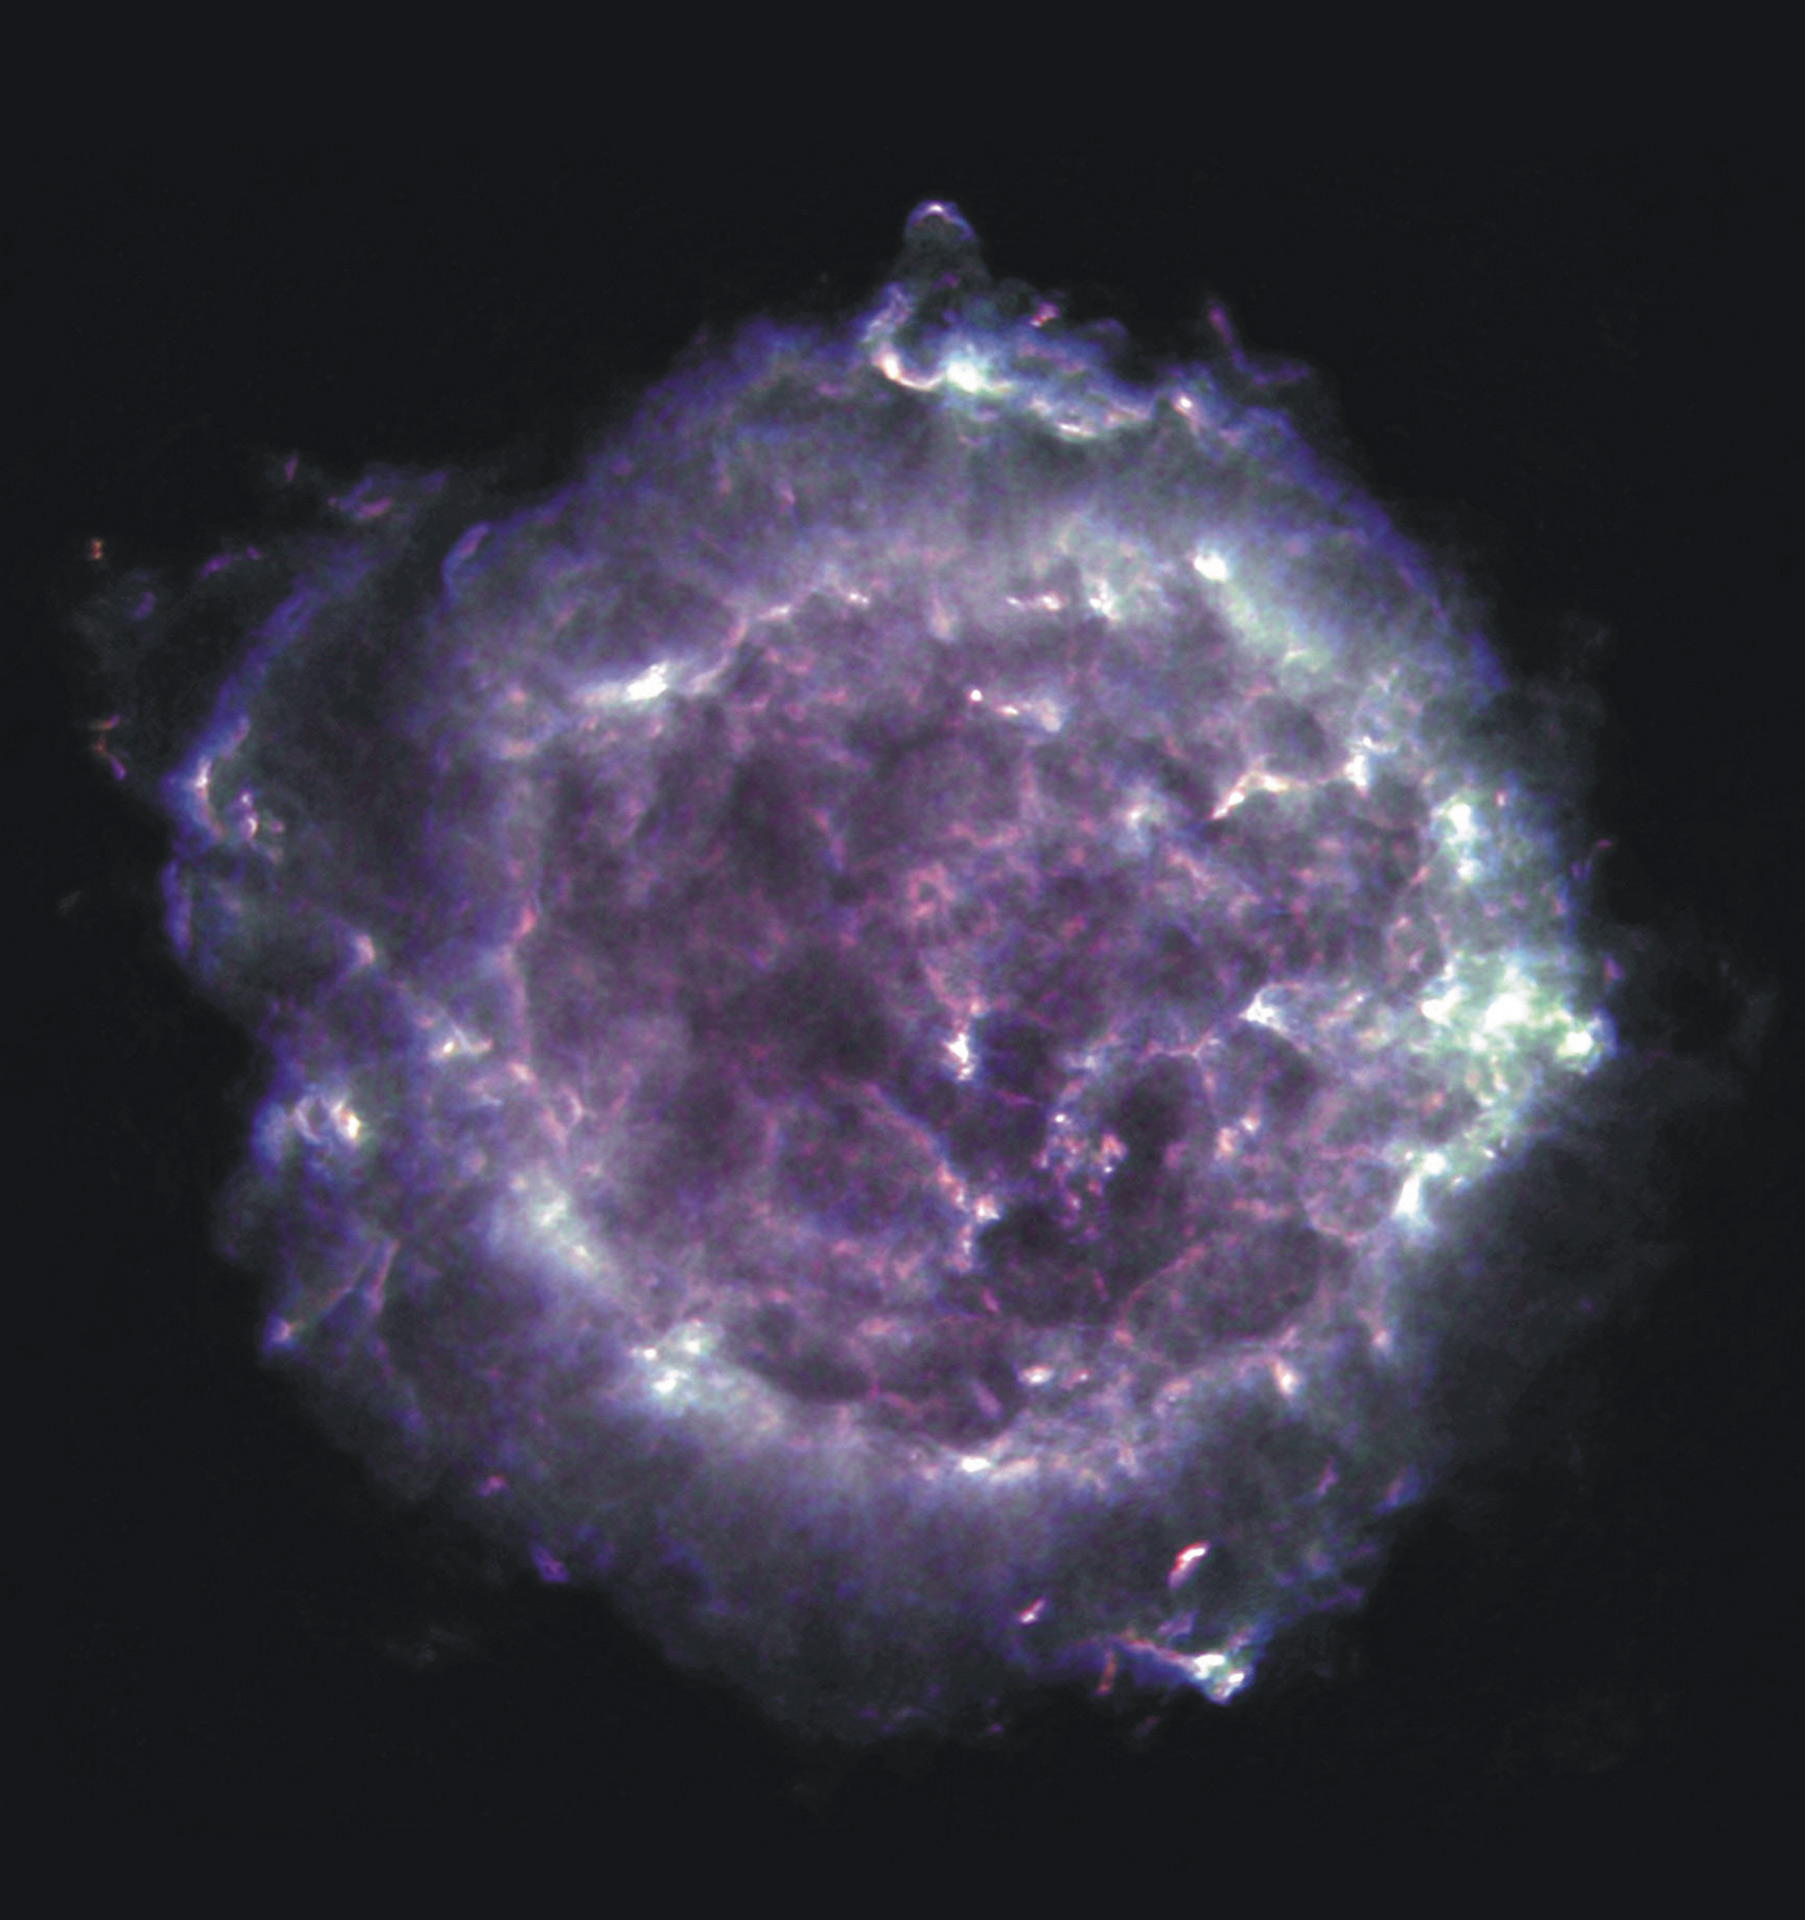
\includegraphics[width=0.6\textwidth]{CassA_2002_large-1_Radio.jpg}
	\caption{
		Изображение остатка Кассиопея А в радиодиапазоне.
	}
	\label{fig:Cas A Radio}
\end{figure}

\indentПосле 1948 г. в нашей Галактике было открыто несколько источников радиоизлучения, связанных с остатками вспышек сверхновых. В 1949 г. австралийскими радиоастрономами было обнаружено радиоизлучение от Крабовидной туманности (рис. \ref{fig:Сrab Nebula Rafio Optic}). Как стало ясно в дальнейшем, Крабовидная туманность является прототипом целого ряда остатков, получивших название "плерионы". Их отличие от классических оболочечных радиоостатков увеличение яркости к центру, плоский спектр, более высокая степень поляризации и более регулярная структура магнитного поля. 
Через 3 года было обнаружено радиоизлучение от остатков вспышек 1572 г. (Тихо)  и 1604 г. (Кеплер). 

\begin{figure}[!htb] 
	\centering
	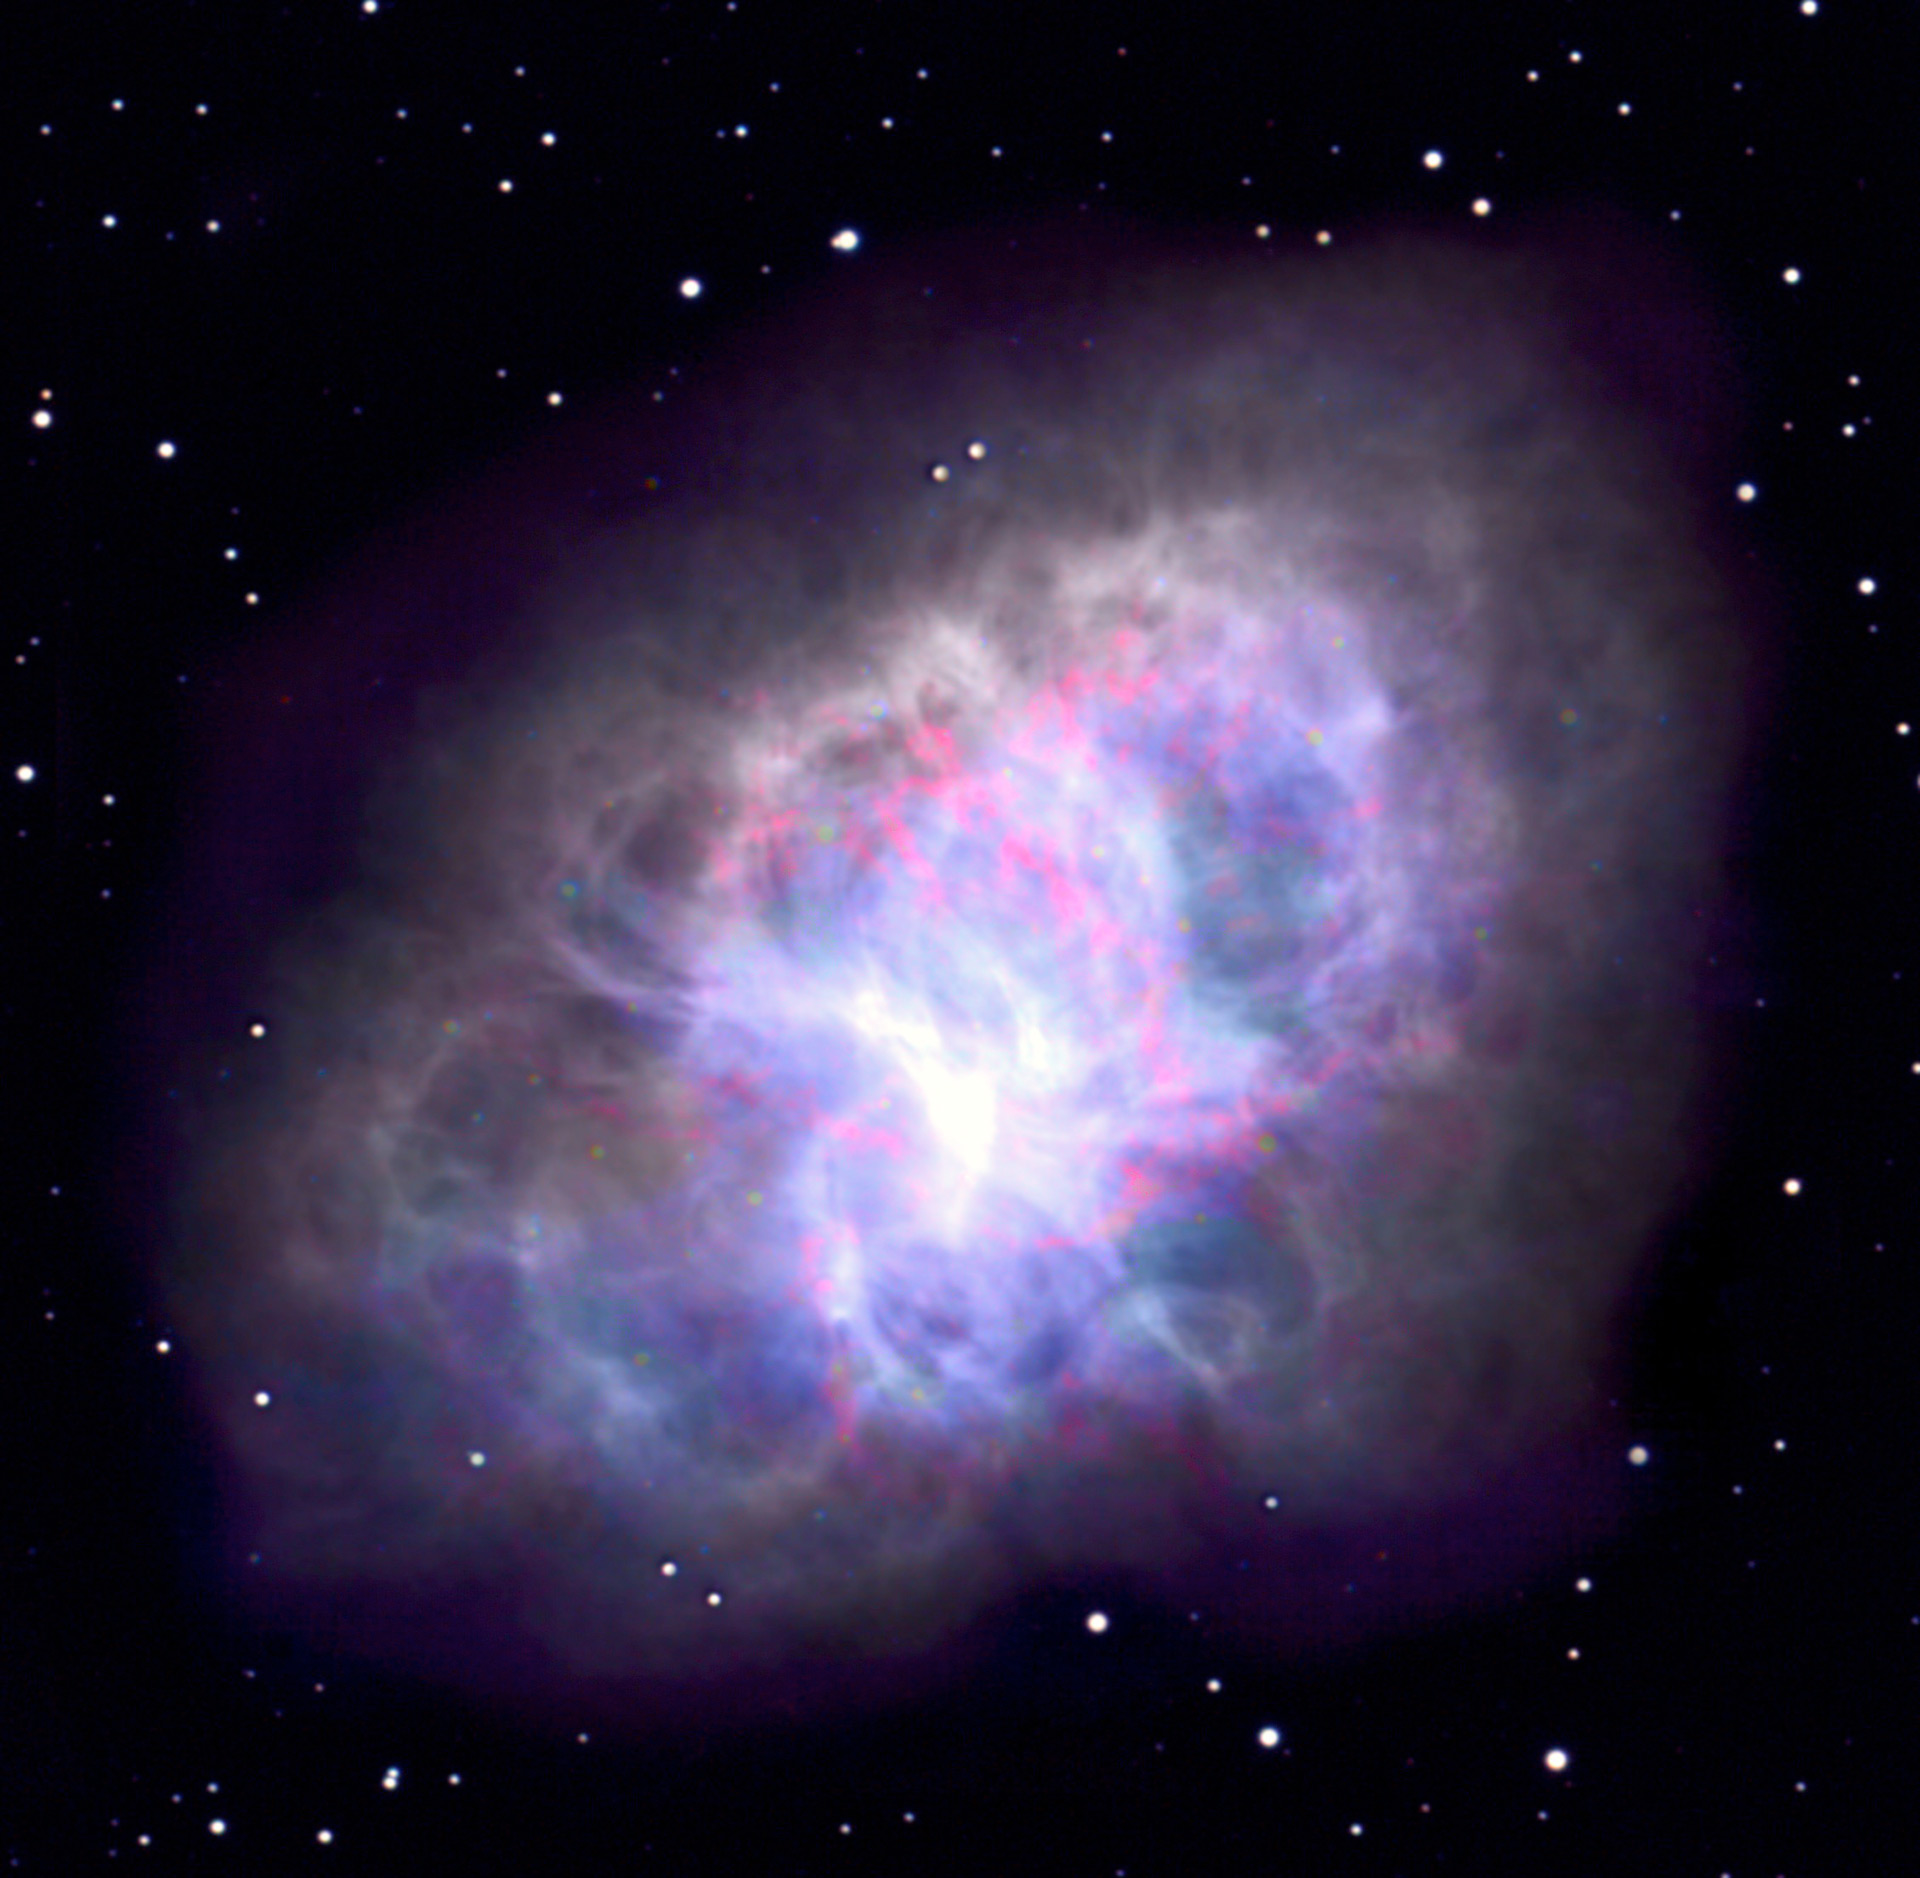
\includegraphics[width=0.6\textwidth]{M1TB2flat_large_Radio_Optic.jpg}
	\caption{
		Изображение Крабовидной туманности в радиодиапазоне (фиолетовый, синий и зеленый) и видимом диапазоне (красные линии) 
	}
	\label{fig:Сrab Nebula Rafio Optic}
\end{figure}


Радиоизлучение в космическом пространстве может появляеться по разным причинам.
К механизмам его возникновения относятся: тепловое радиоизлучение, реликтовое излучение, магнитотормозное (циклотронное и синхротронное) радиоизлучение, радиоизлучение плазмы, рекомбинационное (линейчатое) радиоизлучение, мазерное излучение молекул. \cite{Kaplan1966}
В остатках сверхновоых основным механизмом является синхротронный. В следубщем разделе приводится детальное описание этого механизма.
\subsection{Синхротронное излучение} \label{sec: Synchrotron}
Синхротронное излучение имеет магнитотормозную природу, но отличается от циклотронного тем, что частицы здесь являются релитивистскими, соотвественно их энергии много больше. 
Для описания движения таких частиц используются законы теории относительности. Далее приводятся некоторые основные формулы и характеристики, описывающие данный тип излучения. 
Для частиц движущихся со скоростями $v$ близкими к скорости света $с$ энергия задается формулой: $$E = m_0c^2\cdot \gamma,$$ где $\gamma = {1/\sqrt{1-v^2/c^2}}$ - фактор Лоренца, $m_0$-масса неподвижной частицы. Также при движении тела его размер в направлении движения сокрщается в $\gamma$ раз и во столько же раз замедляется ход времени в нем. 
Как и в случае циклотронного излучения электрон в магнитном поле движется по окружности или по спирали. Для релятивистского электрона: 
$$ \Tilde{f}_H=18\frac{H_{\perp}}{E}\hbox{ \slshape[кГц]},$$
здесь $H_{\perp} = Hcos\theta$ - компонента магнитного поля, перпендикулярная скорости электрона. 
Таким образом, основная частота обращения релятивистского электрона мала; поэтому велика длина волны и "основного тона" его радиоизлучения. Но релятивистский электрон значительно больше энергии излучает на высоких обертонах(гармониках). Неподвижный электрон создает вокруг себя электрическое поле, одинаковое по всем направлениям, а если он движется с ускорением, но медленно, то вместе с ним движется и это сферически симметричное поле. Поэтому медленный электрон излучает более или менее одинаково во всех направлениях. Если же электрон движется очень быстро, то его электрическое поле как бы сплющивается в направлении движения из-за сокращения масштабов. Это означет, что поле особенно сильно меняется в направлении вдоль скорости электрона; отсюда также следует, что релятивистский электрон излучает электромагнитные волны главным образом вперед, по направлению своего движения. 

\begin{figure}[!htb]
	\centering
	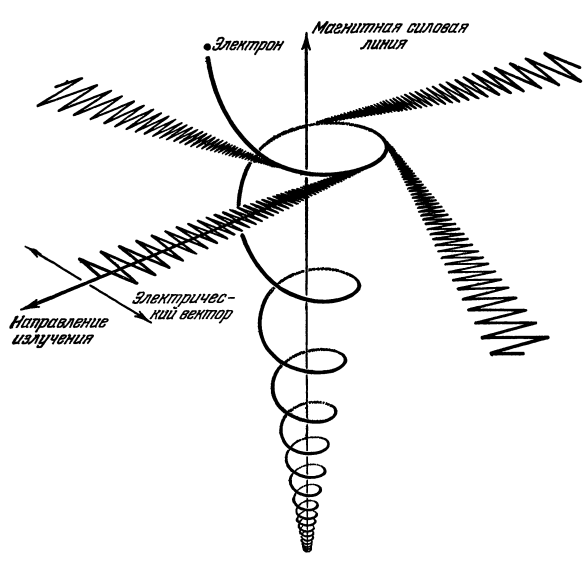
\includegraphics[width=0.5\textwidth]{synchrotron_radiation.png}
	\caption{
		К объяснению синхротронного механизма радиоизлучения.
	}
	\label{fig:synchrotron_radiation}
\end{figure}
Угол раствора конуса, в который излучает релятивистский электрон, по порядку величины (в радианах) равен тому же универсальному отношению 0.51/E (МэВ).

%-------------------------------------
\section{Остатки сверхновых} \label{sec: Supernova remnants}
Перейдем теперь к более подробному рассмотрению процессов, происходящих в разлетающихся остатках.
Сброшенная при вспышке сверхновой оболочка расширяется со сверхзвуковой скоростью в межзвёздную среду и образует ударную волну. 
Различают несколько стадий взаимодействия оболочки с окружающей средой: свободный разлёт, адиабатическое расширение, стадия 
снегоочистителя. Далее идёт более подробное описание каждой из них.({\cite{Spitzer1981}})

\subsection{Стадия 1. Свободный разлёт} \label{sec:free_exp}
На этой стадии оболочка движется по инерции так, как если бы внешней среды не было вообще. $R(t)\propto t $ 
Излучение оболочки не играет роли в ее динамике. Стадия заканчивается при сгребании массы окружающего вещества, равной массе расширяющейся оболочки $M_0 = 4\pi/3\rho_0R^3$. 
Сделаем оценку по порядку величины для характерных значений масс и скоростей разлетающейся оболочки сверхновой.
Для $\rho_0=2\times10^{-24}$\,г/см$^3$, $v=5\cdot10^8$\,см/с и $M_0=1M_{\odot}$ этот момент наступает примерно через 200 лет после начала расширения при $R\approx 2$\,пк.

\subsection{Стадия 2. Адиабатическое расширение} \label{sec: adiabatic_exp}
На этой стадии радиационные процессы по-прежнему динамически неважны, так как температура газа за фронтом ударной волны очень высокая. Кинетическая энергия оболочки расходуется на нагрев газа за фронтом сильной ударной волны и на ускорение сгребённого межзвёздного газа. Когда масса сгребённого газа много больше $M_0$, движение оболочки довольно точно описывается автомодельным решением Л.И. Седова для сильного взрыва в среде. 
Можно получить зависимость поведения радиуса оболочки от времени из простых физических соображений, представленных ниже.

Пусть тепловая энергия газа, находящаяся в равновесии с кинетической, составляет долю $K_1$ от полной энергии $E$, а давление непосредственно за фронтом УВ $p_2$ в $K_2$ раз больше среднего давления внутри оболочки. Для идеального газа с показателем адиабаты $\gamma=5/3$, среднее давление равно $p=(\gamma-1)\epsilon=2/3\epsilon,\  \epsilon$-средняя плотность тепловой энергии, что даёт 
$$p_2=K_2\cdot \frac{2}{3}\cdot \frac{3K_1E}{4\pi R_s^3}=\frac{KE}{2\pi R_s^3},\ \text{где } K=K_1K_2$$
Но в случае сильных ударных волн справедливо соотношение
$$p_2=\frac{2\rho_1u_1^2}{\gamma+1}$$
между давлением сразу за фронтом $p_2$, плотностью $\rho_1$ и скоростью втекания невозмущенного гаща в УВ $u_1$. Комбинирую эти уравнения и учитывая, что $u_1=dR_s/dt$, получаем $$u_1^2=\left(\frac{dR_s}{dt}\right)^2=\frac{2KE}{3\pi \rho_1 R_s^3}$$
Точный динамический расчет дает для $\gamma=5/3$ $K_1=0.72,K_2=2.13$, следовательно, $K=1.53$
Интегрируя последнее уравнение, получаем 
$$R_s(t)=\left(\frac{2.2E}{\rho_1}\right)^{\frac{1}{5}}\cdot t^{\frac{2}{5}}=10^{15} \left(\frac{E}{E_0 n_1}\right)^{1/5} t^{2/5} \text{пк,}$$
где $n_1$ - концентрация атомов в невозмущенной межзвездной среде, время t выражено в годах, $E_0 = 7.5\cdot10^{50}$ эрг.
Поскольку температура за фронтом сильной ударной волны для идеального газа с $\gamma=5/3$
$$T_s = \frac{3\mu}{16k_B}u_1^2=1.8\cdot 10^5 \left(\frac{R}{t} \right)^2\text{кэВ},$$
где $k_B$-постоянная Больцмана, $\mu$ -молекулярный вес,
подставляя в это выражение полученные выше соотношения, получаем, что температура падает со временем, как 
$T \propto R_s^{-3} \propto t^{-\frac{6}{5}}$, начиная с некоторого момента времени (радиуса оболочки) становятся важными процессы радиоактивного охлаждения УВ и адиабатическое приближение нарушается. 
В конце стадии свободного разлета возникает обратная ударная волна, распространяющаяся внутрь оболочки(в системе координат, связанной с фронтом УВ), но движущаяся наружу в лабораторной системе (т.е газ втекает в обратную ударную волну изнутри оболчки). 

\subsection{Стадия 3. Стадия снегоочистителя}
Наступает после катастрофического охлаждения газа оболочки, когда температура падает ниже $\approx 6\times 10^5$ K и плазма начинает интенсивно высвечивать запасенную тепловую энергию. УВ при этом становится изотермической ($\gamma=1$). 
Оболочка становится холодной и тонкой, поскольку скорость газа, прошедшего через ударную волну, меньше скорости движения фронта по среде и газ, поджимаемый давлением оболочки изнутри, долго остается вблизи фронта УВ.

Движение УВ поддерживается за счет запасенного в оболочке импульса ($M(dR_s/dt)=const$, $M=4\pi/3\rho_1R_s^3$. В этом режиме расширение оболочки замедляется, т.к из сохранения импульса следует $dR_s/dt\propto 1/R_s^3$ (а не $R_s^{-3/2}$ как в случае адиабатического разлета). 
%
Переход к этому режиму происходит при радиусе оболочки % \pb{Перенес формулу сюда, после обоснования}
$$R_c=24\left( \frac{E\cdot10^{-51}\hbox{эрг/с}}{n_0}\right)^{\frac{1}{3}}\hbox{пк}$$ 

%---------------------------------------


\newpage
%------------------------------------------------
\section{Заключение}
В ходе работы были изучены основные физические процессы связанные с разлетом остатков сверхновых: 
\begin{itemize}
    \item Во время разлета остаток активно излучает в радиодиапазоне. Особенно сильно это происходит на переднем фронте остатка, на границе с межзвездным веществом. Это связано с тем обстоятельством, что столкновение остатка с окружающим веществом приводит к возникновению ударных волн (резких скачков уплотнения), которые передают огромные скорости частицам газа, что заставляе их излучать.
    \item Синхротронный механизм возникновения радиоизлучения является основным проявляющимся в данной процессе. На границе остатка и окружающего газа возникают сильные завихрения магнитного поля, засчет которого электроны начинают лететь по спиралям и излучать.
\end{itemize}
Процесс выполнения работы включал изучение теоретических материалов, имеющих описание рассматриваемых физических явлений. Цели работы были достигнуты. 
\\ \\
В ходе выполнения работы также была написана программная реализация аналитического решения задачи Римана, позволяющая гораздо лучше понять причины возникновения ударных волн и их основные свойства. В частности, повышение энтропии газа, через который прошла ударная волна.
В дальнейшей работе автором планируется расширить данную программу до случая сферически симметричного распространения ударных волн, который имеет непосредственное отношение к реальным астрофизическим условиям. Также важным этапом дальнейшей работы будет углубленное изучение численных методов применяемых к рассматриваемой задаче. 

\clearpage
\sloppy
\printbibliography
\addcontentsline{toc}{section}{\bibname}
\newpage

%------------------------------------------------
\appendix
\section{Приложение. Ударные волны в ударной трубе}\label{sec: Shockwave}
Для исследования  ударных волн в земных условиях применяют ударные трубы. Классической задачей при исследовании ударных волн является задача Римана о распаде произвольного разрыва в ударной трубе. 
\subsection{Задача Римана о распаде произвольного разрыва}
Формулировка задачи звучит следующий образом: рассматривается одномерная задача с двумя областями с различными идеальными газами, разделённых жесткой перегородкой. Начальные условия у газов различны, слева от перегородки $p_L, u_L, \rho_L$; справа - $p_R, u_R, \rho_R$. В момент $t=0 $ перегородка исчезает (\cite{BulatVolkov2015,zr1968}). 
В следующие моменты времени образуются несколько подобластей с постоянными параметрами, появляющиеся благодрая возникновению в газах волн разных типов: сильных устойчивых разрывов (ударных волн), непрерывных газодинамических течений (волн разрежения). Для описания этих волн выписывается система уравнений, олицетворяющих законы сохранения массы, импульса и энергии. Ниже приводится дифференциальная форма этих уравнений.(\cite{zr1968})
\subsection{Основные гидродинамические уравнениия}
Выпишем систему уравнений газодинамики, определяющих изменение свойств газа: плотность, скорость и давление.
Закон сохранения массы описывается уравнением непрерывности: 
\begin{equation}
    \frac{\partial \rho}{\partial t} + div(\rho \vecxu) = 0 \label{eq:continuity}
\end{equation}
Закон сохранения импульса описывается уравнением Эйлера:
\begin{equation}
    \frac{\partial  \vecxu}{\partial t} + \left(\vecxu \nabla \right)\vecxu = -\frac{1}{\rho}\nabla P  \label{eq:euler}
\end{equation}
И закон сохранения энергии задается уравнением:
\begin{equation}
    \frac{\partial }{\partial t}\rho(E+\frac{\vecxu^2}{2}) + div(\rho \vecxu (w+\frac{\vecxu^2}{2})) = 0  \label{eq:energy} 
\end{equation}
Для полного описания решений этой системы необходимо также задать несколько соотношений.
Одно из них это уравнение состояния:
\begin{equation}
p = p(\rho,e)
\end{equation}
второе выражает закон сохранения энтропии:
\begin{equation} \label{eq:entropy} 
\frac{d s}{d t} = 0
    \quad\text{или}\quad  
\frac{\partial s}{\partial t} + (\vecxu \cdot \nabla)s = 0 
\end{equation}
В случае рассмотрения ударных волн в одномерном ударной трубке, данная система дифференциальных уравнений (\ref{eq:continuity}-\ref{eq:energy}) преобразуется в систему нелинейных алгебраических уравнений. Из которой затем выписываются основные соотношения (соотношения Ранкина-Гюгонио) для гидродинамических величин по разные стороны от фронта ударной волны. Конкретный вид этих соотношений будет приведен ниже (в следующем разделе).

Можно также заметить, что в исходную гидродинамическую систему не входят параметры с размерностями длины и времени, поэтому решение задачи является автомодельным, т.е такое, что переменные x и t входят в него лишь в комбинации \(x/t\).

В зависимости от начальных условий образуется та или иная
конфигурация устойчивых разрывов и непрерывных газодинамических течений (см. рис. 1). Возможные
решения содержат веер волн разрежения(ВР), контактный разрыв(КР) и ударную волну (УВ), разделяющие область
течения на четыре подобласти с постоянными значениями параметров. 
В конфигурации A возникает
ударная волна, контактный разрыв и веер волн разрежения, в конфигурации B – две ударные волны и
контактный разрыв, в конфигурации C – две волны разрежения и контактный разрыв. Условно волны
называют левой и правой волной (в неподвижной системе координат они могут двигаться в одну сторону). В случае ударной волны речь идет о движущемся фронте разрыва, по обе стороны которого параметры газа полагаются постоянными (своими для каждой из сторон) и связанными определенными соотношениями. В случае волны разрежения имеется область переменного течения, в которой параметры газа
остаются постоянными вдоль прямолинейных лучей, играющих роль характеристик системы уравнений,
а значения параметров зависят от наклона в веере характеристик, описывающем волну разрежения. Волна разрежения граничит с областями постоянного течения, подобным тем, которые имеют место для
ударной волны. 

В данной работе в качетсве теста используется задача Сода, начальные условия которой приводят к конфигурации А: ударная волна(справа), контактный разрыв, волна разрженеия(слева).
\begin{figure}[h]
\begin{minipage}[h]{0.32\linewidth}
\center{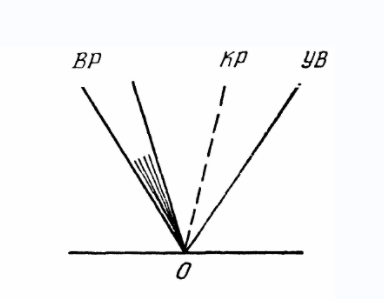
\includegraphics[width=1\linewidth]{Configuration A.png} \\ A}
\end{minipage}
\hfill
\begin{minipage}[h]{0.32\linewidth}
\center{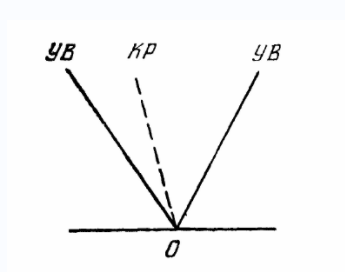
\includegraphics[width=1\linewidth]{Configuration B.png} \\ B}
\end{minipage}
\hfill
\begin{minipage}[h]{0.32\linewidth}
\center{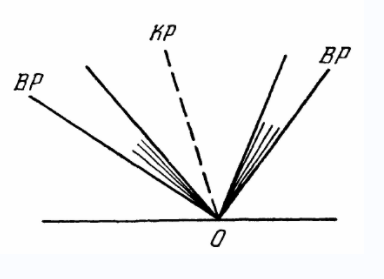
\includegraphics[width=1\linewidth]{Configuration C.png} \\ C}
\end{minipage}
\caption{Возможные конфигурации волн}
\label{fig:Sod 2 moments}
\end{figure}

\subsection{Соотношения на границах областей} \label{sec: relations bound}
В рассматриваемой задаче оба газа являются идеальными, т.е удовлетворяют соответствующему уравнению состояния: $ pV = \nu RT$.

Для них выполнено уравнение для энтропии идеального газа: $S = C_v\log(p/\rho^\gamma)+const$.

Показатель адиабаты обоих газов: $\gamma = 1.4$.

Используются следующие обозначения для состояний газа:
\begin{itemize}
    \item $p_L, u_L, \rho_L$ - начальные условия газа слева (газ, по которому еще не прошла волна разрежения),
    \item $p_1, u_1, \rho_1$ - условия в газе, охваченном волной разрежения,
    \item $p_2, u_2, \rho_2$ - условия в газе между волной разрежения и контактным разрывом (прошла волна разрежения)
    \item $p_3, u_3, \rho_3$ - условия в газе между контактным разрывом и ударной волной (прошла ударная волна)
    \item $p_R, u_R, \rho_R$ - начальные условия газа справа (газ, по которому еще не прошла ударная волна).
\end{itemize}

Решение состоит из соотношений на трех волнах: ударной волне, контактном разрыве и волне разрежения. 
\begin{enumerate}
    \item Для ударной волны. \\
    Соотношения Ранкина-Гюгонио выраженные через число Маха ($M= D/c_1$) выглядят следующим образом:
    \begin{eqnarray}
        \frac{p_3}{p_R} & = & \frac{2\gamma}{\gamma+1}M^2-\frac{\gamma-1}{\gamma+1} \\
        \frac{\rho_3}{\rho_R} & = & \frac{(\gamma+1)M^2}{(\gamma-1)M^2+2} \\
        \frac{u_3}{c_R} & = & \frac{2}{\gamma+1}(M-\frac{1}{M})
    \end{eqnarray} 
    $c_R = \sqrt{\gamma p_R / \rho_R}$  - скорость звука в среде перед фронтом, $D$ - скорость ударной волны.
    
    Формула адиабаты Ранкина-Гюгонио:
    \begin{align}
        \frac{p_3}{p_R}=\frac{\rho_3(\gamma+1)-\rho_R(\gamma-1)}{\rho_R(\gamma+1)-\rho_3(\gamma-1)}
    \end{align}

    \item Для контактного разрыва.
    Давление и скорость газа не меняются на контактном разрыве. 
    \begin{eqnarray}
        p_2 &=& p_3\\
        \rho_2 &=& \rho_L \left( \frac{p_3}{p_L} \right)^\frac{1}{\gamma}\\
        u_2 &=& u_3
    \end{eqnarray} 
    \item Для волны разрежения.
    В волне разрежения параметры убывают непрерывно, в отличие от ударных волн.
    \begin{eqnarray}
        p_1(x,t)&=&p_L \left( 1-\frac{\gamma-1}{2}\frac{u_1(x,t)}{c_L} \right)^\frac{2\gamma}{\gamma-1},\\
        \rho_1(x,t)&=&\rho_L \left( 1-\frac{\gamma-1}{2}\frac{u_1(x,t)}{c_L} \right)^\frac{2}{\gamma-1},\\
        u_1(x,t) &=& \frac{2}{\gamma+1}(c_L + \frac{x}{t}).
    \end{eqnarray} 
\end{enumerate}

\indent Конкретные значения параметров $p_2,u_2$ при заданных начальных условиях получаются из решения системы нелинейных алгебраических уравнений, благодаря равенству параметров слева и справа от контактного разрыва.

\subsection{Тест Сода}
На рис.\ref{fig:Sod 2 moments} представлены графики параметров газа($p,\rho,u, S, T$) в начальный момент времени ($t=0$) и момент $t=0.2$ при начальных условиях задачи Сода: 
\begin{equation}
        (p, u, \rho) =
        \begin{cases}
            (1.0, 0.0, 1.0), & \text{при } -1\leq x\leq0,\\
            (0.1, 0.0, 0.125), & \text{при } 0\leq x\leq1.
        \end{cases}
\end{equation}

\begin{figure}[h]
\begin{minipage}[h]{0.49\linewidth}
\center{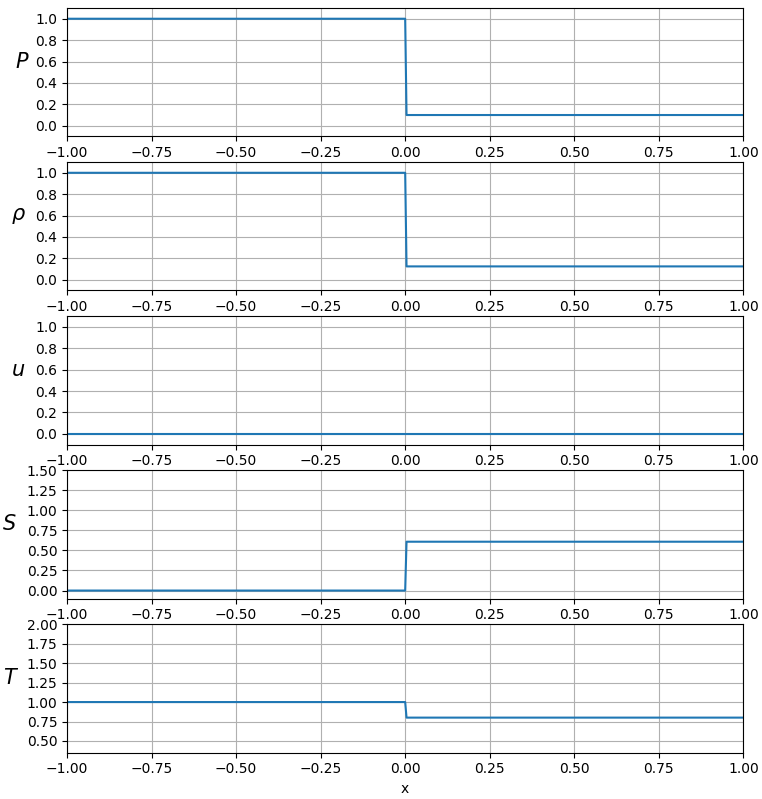
\includegraphics[width=1\linewidth]{Initial_Sod.png} \\ а)}
\end{minipage}
\hfill
\begin{minipage}[h]{0.49\linewidth}
\center{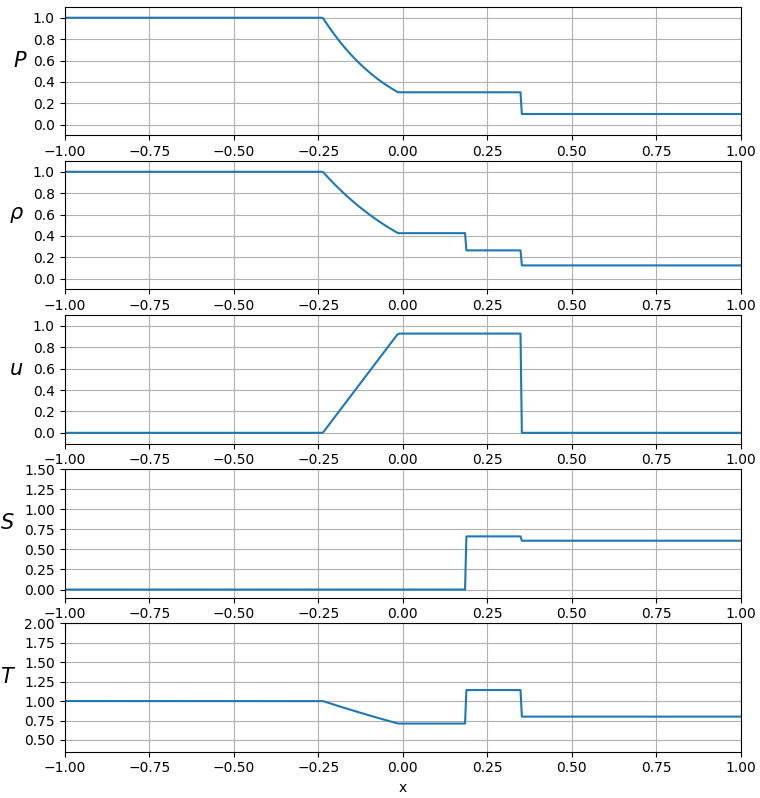
\includegraphics[width=1\linewidth]{t_02_Sod.png} \\ б)}
\end{minipage}
\caption{Параметры газа a) в начальный момент $t=0$ cек б) в момент $t=0.2$ сек}
\label{fig:Sod 2 moments}
\end{figure}
%------------------------------------------------

%-------------------------------------------------


\end{document}
